\documentclass[10pt]{article}

\usepackage{rlc}
% If accepted, instead use the following line for the camera-ready submission:
%\usepackage[accepted]{rlc}
% To de-anonymize and remove mentions to RLC (for example, for posting to preprint servers), instead use the following:
% \usepackage[preprint]{rlc}

\usepackage{array}
\usepackage{amsmath}
\usepackage{amsthm}
\usepackage{amsbsy}
\usepackage{amssymb}
\newtheorem{definition}{Definition}
\usepackage{graphicx}
\usepackage{mathtools}
\usepackage{nicefrac}
\usepackage{bm}
\usepackage{enumitem}
\usepackage{mpemath}
\usepackage{tcolorbox}
\usepackage[capitalize,noabbrev]{cleveref}
\usepackage{theoremref}
\usepackage{thmtools}
\usepackage{thm-restate}
\usepackage{algorithm}
\usepackage{algpseudocode}
\usepackage{tikz}

\bibliographystyle{abbrvnat}
\usepackage[framemethod=default]{mdframed}

\renewcommand{\cite}{\citep}

%\mathtoolsset{showonlyrefs}     % Only number equations that are referenced (optional)

\renewcommand{\algorithmicrequire}{\textbf{Input:}}
\renewcommand{\algorithmicensure}{\textbf{Output:}}


\theoremstyle{plain}
\newtheorem{theorem}{Theorem}
\newtheorem{lemma}{Lemma} 
\newtheorem{proposition}{Proposition}
\newtheorem{assumption}{Assumption}
\theoremstyle{remark}
\newtheorem{example}{Example}

\newcommand{\mm}[1]{\textcolor{magenta}{[#1]}}
\newcommand{\db}[1]{\textcolor{blue}{[DB: #1]}}
\newcommand{\gersi}[1]{\textcolor{red}{[#1]}}
\newcommand{\s}[1]{\mathcal{#1}}

\DeclareMathOperator{\ext}{ext}

% \setlength{\parskip}{3mm plus 1mm minus 1mm}
% \setlength{\parindent}{0pt}

\title{ROIL: Robust Offline Imitation Learning\\
  without Trajectories}
\author{Gersi Doko \\
        Gersi.Doko@unh.edu \\
        \and 
        Daniel Brown \\
        Marek Petrik \\
        mpetrik@cs.unh.edu 
      }

% Relevant emails
% Daniel Brown = daniel.s.brown@utah.edu
% Guang = u1326446@utah.edu

\begin{document}

\maketitle

\begin{abstract}
We study the problem of imitation learning via inverse reinforcement learning where the agent attempts to learn an expert's policy from a dataset of collected state, action tuples. We derive a new robust model-based offline Imitation Learning method (ROIL) that mitigates covariate shift by avoiding estimating the expert's occupancy frequency. Frequently in offline settings, there is insufficient data to reliably estimate the occupancy frequency and this leads to models that do not generalize well. Our proposed approach, ROIL, a method that is guaranteed to recover the experts occupancy frequency and is efficiently solvable as an LP. We demonstrate ROIL's ability to perform well in a large grid world environment even under large covariate shift such as when the state visitation frequency of the demonstrations does not come from the expert.
\end{abstract}

\section{Introduction}

\emph{Imitation learning} seeks to compute a good policy in a Markov decision process~(MDP) without knowing the reward function. Instead, one only has access to a set of demonstrations performed by a domain expert~\cite{chang2021mitigating, Panaganti2023, Spencer2021, Rashidinejad2022}. Imitation learning promises techniques that can learn to act well in environments where describing an appropriate reward function may be challenging or impractical. Robotics, medicine, and autonomous driving and examples of problem domains that can benefit greatly from more reliable imitation learning algorithms. 

Inverse Reinforcement Learning~(IRL), or apprenticeship learning, is a common approach to imitation learning~\cite{abbeel2004, ziebart2008maximum, Brown2018a, fu2018learning}. IRL leverages the environment's dynamics modeled as an MDP to efficiently mimic the observed policy of the expert~\cite{arora2021survey}. The environment's dynamics may be known a priori~\cite{Syed2008, lacotte2019} or estimated from data~\cite{Ho2016,chang2021mitigating}. An important strength of IRL algorithms is that they can learn to mimic experts quite well even with remarkably little data. However, most IRL algorithms can be very sensitive to the state distribution in the training data. If the distribution of states present in the dataset does not follow the occupancy frequency---a phenomenon known as \emph{covariate shift}---the IRL algorithm may compute a policy that is much worse than the expert's policy. 

In this paper, we propose ROIL, a new approach to IRL that is particularly resistant to any covariate shift. In particular, ROIL allows for data with a state distribution that does not follow the expert's occupancy frequency. Most existing algorithms are sensitive to covariate shifts because, in some form, they reduce to matching the expert's state occupancy frequency. In comparison, ROIL attempts to recover the set of plausible expert policies from the training data and compute a policy that minimizes the regret with respect to this set of experts. With an appropriate choice of modeling assumption, we show that ROIL can be formulated as a convex optimization problem and solved using mature solvers.

There are several reasons for why the expert demonstration data may not be sampled according to the true occupancy frequency. First, the expert's initial state distribution may differ from the initial state distribution when the learned policy is deployed. Second, the expert may focus on providing pedagogic demonstrations that focus on the most challenging parts of the state space~\cite{cakmak2012algorithmic,hadfield2016cooperative,Brown2018b}. Third, the demonstrations may not even form a trajectory but instead consist of disconnected state-action pairs. Finally, the state distribution of the demonstrations may differ simply due to sampling and model errors and inconsistencies. These demonstrations can be noisy and may not be representative of the expert's true policy. As a result, one must be careful in solving the primal IL formulation to make it tractable.

To better illustrate the importance of covariate shift, consider the following extreme example. In an MDP with a small state space and the ability to jump between states, the expert provides a single demonstration for each state showing the optimal actions. Behavior cloning algorithms, which reduce imitation learning to a classification problem, will recover the optimal policy given that the classification bias is general enough. Yet, most common IRL algorithms based on the same scheme as LPAL~\cite{Syed2008} or GAIL~\cite{Ho2016} can fail to recover a good policy, as we show below. ROIL, on the other hand, recovers the optimal policy even in this extreme setting while preserving most of the benefits of the low sample complexity of IRL.

ROIL builds on the same ideas as most modern IRL algorithms and can be readily integrated with the improvements developed in recent years~\cite{arora2021survey}. As with most IRL algorithms, ROIL seeks to minimize the regret to the expert's policy for the worst-case plausible reward functions. However, ROIL departs significantly from existing IRL algorithms in that it does not directly use the estimate of expert's occupancy frequencies. In contrast, ROIL uses the training data to construct a robust set of plausible expert policies and minimizes the regret of the computed policy in the context of this set. As a result, ROIL cannot be seen as matching the expert's feature frequencies, which is a popular view of existing IRL techniques~\cite{abbeel2004,Syed2008,Ho2016}.


The remainder of the paper is organized as follows. \Cref{sec:preliminaries} describes the background in MDPs and IRL necessary to introduce ROIL. Then, in \cref{sec:optimization-formulation}, we describe our general framework, analyze its basic properties, propose an optimization algorithm, and discuss several practical extensions. \Cref{sec:theoretical-analysis} analyzes ROIL's guarantees and limitations theoretically and compares them with prior work. Finally, in \cref{sec:experimental-results}, we analyze ROIL numerically and compare it with relevant algorithms. 

\section{Preliminaries}\label{sec:preliminaries}

Before describing the underlying MDP framework and formally defining the IRL problem, we define the basic notation we use in the paper. We use calligraphic letters to denote sets and a tilde to denote random variables. We also adopt the standard convention that $\mathcal{A}^{\mathcal{B}}$ represents the set of all functions from a set $\mathcal{B}$ to a set $\mathcal{A}$ and treat vectors as function from indexes to real numbers. Finally, the sets $\Real$ and $\Real_+$ represent real and non-negative numbers respectively. 


%This introduction is not meant to be exhaustive, but rather to provide the reader with the necessary background to understand the rest of the paper.
%Much of the MDP material comes from~\cite{Puterman1994}.
%For a more in-depth treatment of the IRL setting we refer the reader to~\cite{abbeel2004}.

% \paragraph{Markov Decision Processes}

We assume that the domain can be modeled as a \emph{Markov Decision Process}~\cite{Puterman1994} with a finite number of states $\mathcal{S} = \left\{ 1, \dots , S \right\}$ and a finite number of actions $\mathcal{A} = \left\{ 1, \dots , A \right\}$. The transition probability function $p\colon \mathcal{S} \times \mathcal{A} \to \Delta^{\mathcal{S}}$, where $\Delta^{\mathcal{S}} = \left\{ x\in \Real_{+}^S \mid \sum_{s\in \mathcal{S}} x_s =1 \right\}$ is the probability simplex over the elements of the set $\mathcal{S}$. The reward function $r\opt \colon \mathcal{S} \times \mathcal{A} \to \Real$ represents the reward obtained in each transition. We assume that the initial distribution over $p_0\in \Delta^S$ satisfies that $p_0 > 0$.

A solution to an MDP is a \emph{policy}. In this work, we restrict our attention to \emph{stationary randomized} and \emph{deterministic} policies. The set of deterministic policies is $\Pi_{\mathrm{D}}= \mathcal{A}^{\mathcal{S}}$ and the set of randomized policies is $\Pi_{\mathrm{R}} = {\left(\Delta^{\mathcal{A}}\right)}^{\mathcal{S}}$. Note that randomized policies are a special case of deterministic policies. 

%We consider the $\gamma$-discounted infinite horizon objective with $\gamma \in [0,1)$. The infinite-horizon discounted return of a policy $\pi \in \Pi$ and a reward $r \in \mathcal{R}$ is denoted by $\rho(\pi, r)$. 

%The set of deterministic policies is $\Pi_D= \mathcal{A}^{\mathcal{S}}$ and the set of randomized policies is $\Pi_{\mathrm{R}} = {\left(\Delta^{\mathcal{A}}\right)}^{\mathcal{S}}$. The set of all policies is $\Pi = \Pi_{\mathrm{R}} \cup \Pi_D$.

The objective in this work is the $\gamma$-discounted infinite horizon objective with $\gamma \in [0,1)$. We denote the  infinite-horizon discounted \emph{return} of a policy $\pi \in \Pi$ and a reward $r \in \mathcal{R}$ is denoted by 
\[
  \rho(\pi, r)
  \;=\; \lim_{T\to\infty} \mathbb{E}^{\pi, p_0} \left[   \sum_{t=0}^{T} \gamma^t r(\tilde{s}_t,\tilde{a}_t)) \right], 
\]
where the superscript on the expectation indicates that $\tilde{s}_0 \sim p_0$ and $\tilde{s}_{t+1} \sim p(\tilde{s}_t,\tilde{a}_t, \cdot)$, and $\tilde{a}_t \sim \pi(\tilde{s}_t, \cdot )$.  The return $\rho$ is parametrized by the reward because in the IRL setting, the reward is uncertain. 


It will be convenient to treat functions that map states and actions to real numbers as vectors, such as the reward function $r\opt \in \Real^{S \times  A}$. We also use $P_{\pi} \in \Real_+^{S \times S}$ and $r_{\pi}\in \Real^S$  to represent the transition probability matrix and reward vector respectively for each policy $\pi\in \Pi$. Similarly, $P_a$ and $r_a$ represent the transition probability matrix and a reward vector respectively for each action $a\in \mathcal{A}$.

An important and well-known fact that we use is the relation between the occupancy frequencies and policies. In particular, for each policy $\pi\in\Pi_{\mathrm{R}}$ there exists an occupancy frequency $u^{\pi}\in \Real^{\mathcal{S}\times \mathcal{A}}$ such that $\rho(\pi, r) = r_{\pi}\tr u^{\pi}$. The space of occupancy frequencies for all $\pi\in \Pi_{\mathrm{R}}$
is denoted as $\mathcal{U}$ and satisfies~\cite[Section~6.9]{Puterman1994}:
\begin{equation} \label{eq:definition-u}
  \mathcal{U}
  \; =\; 
\left\{ u^{\pi} \mid  \pi \in \Pi \right\}
\; =\;
\Bigl\{ u\in \Real^{SA}_{+} \mid \sum_{a\in \mathcal{A}} (I - \gamma\cdot P\tr_a) \cdot u(\cdot, a) = p_0 \Bigr\}.
\end{equation}
Finally, for each $u\in \mathcal{U}$, one can construct a policy $\pi_u$ such that $u^{\pi} = u$~\cite[Theorem~6.9.1]{Puterman1994} as
\begin{equation}\label{eq:policy-construction}
\pi_u(s, a) \; =\;  \frac{u(s,a)}{\sum_{a' \in \mathcal{A}} u(s,a')}, \qquad \forall s\in \mathcal{S}, a\in \mathcal{A}.
\end{equation}
The policy $\pi_{\mathrm{u}}$ is well-defined because $p_0 > 0$ guarantees that $\sum_{a\in \mathcal{A}} u(s,a) > 0$ for each $s\in \mathcal{S}$.

%\paragraph{Inverse Reinforcement Learning}

With the definitions above, we are now ready to describe the general IRL framework~\cite{abbeel2004,Syed2008,Ho2016}. Recall that the main goal is to learn to act in an environment without knowing the true reward function $r\opt$. Instead, we have access to transition data generated from an expert's policy $\pi_{\mathrm{e}} \in \Pi_{\mathrm{D}}$. To simplify the exposition, we assume that the expert follows a deterministic policy and we discuss generalizations to randomized policies in \cref{sec:optimization-formulation}. The IRL algorithm has access to a dataset  \( \mathcal{D} = {(s_i, \pi_e(s_i))}_{i=1}^D \), where the states may or may not be selected sequentially from state trajectories.

To generalize from a small set of demonstrations, IRL algorithms typically rely on a feature function $\phi\colon \mathcal{S} \times \mathcal{A}\to \Real^k$ that assigns $k$ features to each state and action~\cite{abbeel2004,Syed2008,Brown2018a,lacotte2019,chang2021mitigating,jonnavittula2021know,arora2021survey}. The features $\phi$ represent characteristics of the state-action pair that can determine the reward associates with them. We can represent our features with a feature matrix $\Phi \in \Real^{SA\times k}$ where each row represents the features of a specific state and action. Linear IRL algorithms assume that rewards can be expressed as a linear combination of state and action features. Formally, the set $\mathcal{R} \subseteq \Real^{SA}$ of \emph{feasible rewards} is defined as
\begin{equation} \label{eq:r-defintion}
  \mathcal{R} = \left\{ \Phi w \mid  w\in \mathcal{W} \right\}, \quad
  \text{where} \quad
  \mathcal{W} = \left\{ w \in \Real^k \mid \| w \|_1 \le 1 \right\}. 
\end{equation}
The $L_1$ norm in the definition of $\mathcal{W}$ serves to normalize $w$ because optimal policies are invariant to the scale of the rewards~\cite{abbeel2004,Syed2008}. 

Most IRL algorithms adopt the following scheme. The true reward $r\opt$ is unknown but is assumed to satisfy that $r\opt \in \mathcal{R}$. Algorithms as varied as LPAL~\cite{Syed2008}, GAIL~\cite{Ho2016}, and MILO~\cite{chang2021mitigating} seek to compute a policy that minimizes the worst-case regret with respect the expert's policy. In its essence the regret minimization problem is usually formalized as
\begin{equation} \label{eq:IRL_formulation}
\min_{\pi \in \Pi} \max_{r \in \mathcal{R}} \; \Bigl( \rho(\hat{\pi}_{\mathrm{e}}, r) - \rho(\pi, r) \Bigr).
\end{equation}
Here, $\hat{\pi}_{\mathrm{e}}$ is the empirical estimate of the expert policy $\pi_{\mathrm{e}}$ constructed from the dataset $\mathcal{D}$.

The conceptual optimization in~\eqref{eq:IRL_formulation} is impractical because the optimization over $\pi$ is non-convex and computationally challenging. Instead, using the correspondence between policies and occupancy frequencies in~\eqref{eq:policy-construction}, LPAL and related algorithms solve the following surrogate optimization problem:
\begin{equation} \label{eq:irl-formulation-u}
  \min_{u\in \mathcal{U}} \max_{r\in \mathcal{R}} \, \left(\hat{u}_{\mathrm{e}}\tr r - u\tr r \right)
  \; =\; 
  \min_{u\in \mathcal{U}} \, \left\| \Phi\tr  (\hat{u}_{\mathrm{e}} - u) \right\|_{\infty},
\end{equation}
where the equality follows because $L_{\infty}$ is the dual norm to the $L_1$ norm used in the defintion of $\mathcal{W}$. The value $\hat{u}_{\mathrm{e}}$ represents the \emph{empirical} occupancy frequency approximating $u_{\mathrm{e}}$. Note that the dataset $\mathcal{D}$ is used to estimate the value $\Phi\tr \hat{u}_{\mathrm{e}}$ directly which is also referred to as the \emph{feature counts}.

Some IRL algorithms, like GAIL, add other regularization terms to the scheme in~\eqref{eq:irl-formulation-u} and use $\phi$-divergence based set $\mathcal{W}$. In this work, we do not consider these extensions in order to focus on the fundamental properties and tradeoffs of this formulation.

An important limitation of the formulation in~\eqref{eq:irl-formulation-u} is that it relies on estimating the expert's occupancy frequency $\hat{u}_{\mathrm{e}}$ well. Because the occupancy frequency represents the frequency of \emph{both} states and actions it is very sensitive to the initial distribution and covariate shifts in state distributions which may often arise in imitation learning settings. As discussed in the introduction, the expert may focus on difficult states when performing the demonstrations. In the remainder of the paper, we build on~\eqref{eq:irl-formulation-u} to address its sensitivity to the initial distribution. 

%Non-sequential, in this context, means that the dataset $\mathcal{D}$ may have state, action tuples where $s_{t+1}$ is not distributed accoding to $P(\cdot | s_t, a_t)$. 


% The core of most IRL algorithms is to solve the following optimization problem which minimizes the tobust regret with respect to the occupancy frequency of the expert. 
% \begin{equation} \label{eq:IRL_formulation}
% 	\min_{\pi \in \Pi} \max_{r \in \mathcal{R}} \; (\rho(\pi_{\mathrm{e}}, r) - \rho(\pi, r)),
% \end{equation}
% where $\Pi$ is the set of all policies with $\pi_{\mathrm{e}} \in \Pi$, $\mathcal{R}$ is the set of all reward functions, and $\rho$ is the $\gamma$ discounted 
% \section{Optimization Formulation}\label{sec:optimization-formulation}

% We assume that the true reward function can be written as a linear combination of the features $\Phi$ which are known.

% We will focus on the robust IRL problem, where there is an inner maximization over $\Pi$, see \cref{sec:optimization-formulation}.

\section{ROIL Formulation}\label{sec:optimization-formulation}

% We begin by stating the general formulation of the IRL problem.
% \begin{equation}
% 	\min_{\pi \in \Pi} \max_{r \in \mathcal{R}} \; (\rho(\pi_{\mathrm{e}}, r) - \rho(\pi, r)),
% \end{equation}
% where $\Pi$ is the set of all policies with $\pi_{\mathrm{e}} \in \Pi$, $\mathcal{R}$ is the set of all reward functions, and $\rho$ is the $\gamma$ discounted infinite horizon
% return of a policy given some reward function. This setting is useful for domains where the reward function is hard to define, 
% but features and demonstrations are available. Such domains include robotics, medicine, and autonomous driving. 
% We will focus on the robust IRL problem, where there is an inner maximization over $\Pi$, see \cref{sec:optimization-formulation}.

In this section, we describe and justify ROIL and study its computational properties; we defer the analysis of its approximation errors to \cref{sec:theoretical-analysis}. First, we describe the foundations of the approach in \cref{sec:basic-formulation} and then outline several modifications that reduce ROIL's conservativeness and improve its performance in \cref{sec:incorp-addit-constr}. We conclude the section with a visualization of ROIL as a Chebyshev center problem, which offers additional insights into its performance in \cref{sec:geom-intu-reduct}.  


\subsection{Basic Formulation}
\label{sec:basic-formulation}

Similarly to the standard IRL schema outlined in~\eqref{eq:irl-formulation-u}, ROIL also adopts a principled robust optimization perspective and minimizes the worst-case regret.  The main idea is to compute a policy $\pi\in \Pi$ that minimizes regret with respect to the worst-case plausible expert's policy $\pi_{\mathrm{e}} \in \Pi_{\mathrm{R}}(\mathcal{D})$ and a reward function $r\in \mathcal{R}$. Formally, the basic ROIL optimization problem is as follows:
\begin{equation}
\label{eq:robust_IRL_formulation}
\min_{\pi \in \Pi}  \max_{\pi_{\mathrm{e}} \in \Pi_{\mathrm{R}}(\mathcal{D})} \max_{r \in \mathcal{R}} \,
\left(\rho(\pi_{\mathrm{e}}, r) - \rho(\pi, r)\right).
\end{equation}
Here, $ \Pi_{\mathrm{R}}(\mathcal{D}) \subseteq \Pi_{\mathrm{R}}$ represents the set of all policies consistent with $\mathcal{D}$ and are defined as 
%
\begin{equation} \label{eq:consistent-policies}
\Pi_{\mathrm{R}}(\mathcal{D}) = \left\{ \pi \in \Pi_{\mathrm{R}} \mid \pi(s,a) = 1, \, \forall (s,a) \in \mathcal{D} \right\}.
\end{equation}
We include randomized policies in $\Pi_{\mathrm{R}}(\mathcal{D})$ primarily for notational convenience. Restricting the set of consistent policies to deterministic policies only would not affect the optimal solutions to~\eqref{eq:robust_IRL_formulation}.

If the expert demonstrations in $\mathcal{D}$ are constructed from a deterministic policy, then that policy must be contained in~\eqref{eq:consistent-policies}. However, when the expert's policy is randomized, the construction in~\eqref{eq:consistent-policies} may exclude the expert policy from $\Pi_{\mathrm{R}}(\mathcal{D})$. We discuss how the definition can be extended to account for randomized policies in \cref{sec:incorp-addit-constr}. 

Before describing an efficient formulation for solving ROIL, we discuss its benefits compared with the generic IRL scheme in~\eqref{eq:IRL_formulation}. Recall that the estimated $\hat{u}_{\mathrm{e}}$ in~\eqref{eq:irl-formulation-u} depends on the initial state distribution which may lead to large errors when the demonstration and execution state distributions differ. Instead, ROIL uses the training data to construct the set $\Pi_{\mathrm{R}}(\mathcal{D})$---which is independent of the state distribution---and minimizes regret to all consistent expert policies. 

Next, we show that the ROIL optimization problem in~\eqref{eq:robust_IRL_formulation} can be reduced to a linear program with a polynomial size. It may be surprising that such a reduction is possible since ROIL's objective involves maximizing a non-concave bilinear function. We derive this reduction using the occupancy-based formulation, similar to existing IRL algorithms. A key part of the formulation is a set of occupancy frequencies $\Upsilon$ that are consistent with expert demonstrations defined for $c\in \Real^{SA}$ as 
%
\begin{equation}\label{eq:consistent-occupancies}
  \Upsilon = \left\{ u \in \mathcal{U} \mid c\tr u = 0  \right\},
  \quad
  \text{ where }
  \quad
  c(s,a) =
  \begin{cases}
    1 &\text{if  }
        (s,a) \notin \mathcal{D} \wedge
        \exists a'\in \mathcal{A}, (s, a') \in \mathcal{D}, \\
    0 & \text{otherwise}.
  \end{cases}
\end{equation}

% Now we illustrate the robust IRL learning problem as an optimization problem over the policy and reward space. Then we simplify it using occupancy frequencies
% and the fact that the reward function is linearly realizable by $\Phi$. This allows us in the following section to formulate the problem as a linear program.

% Recall the IRL objective.
% \begin{equation}
% 	\min_{\pi \in \Pi} \max_{r \in \mathcal{R}}  \, (\rho(\pi_{\mathrm{e}}, r) - \rho(\pi, r)),
% \end{equation}


The following lemma shows that the set of occupancy frequencies constructed in~\eqref{eq:consistent-occupancies} is exactly the set of frequencies of policies that are consistent with the dataset. 
\begin{restatable}{lemma}{lemmaOccupancyExistance}
\label{lemma:occ_freq_matching}
If $\mathcal{D}$ are generated by a deterministic policy $\Pi_{\mathrm{D}}$. Then
\[
  u \in \Upsilon
  \qquad \Leftrightarrow \qquad
  \left(u = u^{\pi},\;  \exists \pi \in \Pi_{\mathrm{R}}(\mathcal{D})\right).
\]
\end{restatable}

We now outline the main step in constructing a linear program formulation for solving ROIL. As \cref{lemma:occ_freq_matching} shows,  maximizing over the policy space is equivalent to maximizing over the occupancy frequency space. Then, using the fact that $\rho(\pi,r) = r\tr u^{\pi}$ and the representation of $\mathcal{R}$ in~\eqref{eq:r-defintion}, we can reformulate~\eqref{eq:robust_IRL_formulation} to
%
\begin{equation} \label{eq:roil-occupancy}
    \min_{u \in \mathcal{U}} \max_{r \in \mathcal{R}} \max_{v \in \Upsilon} \, (v- u )\tr  r
    \; =\; 
    \min_{u \in \mathcal{U}} \max_{w \in \mathcal{W}} \max_{v \in \Upsilon} \, (v - u)^T \Phi w.
\end{equation}
%

Solving the formulation in~\eqref{eq:roil-occupancy} directly is challenging because it involves maximizing a non-concave bilinear function in both $w$ and $v$. To turn this optimization into a tractable convex optimization problem, we take the following steps. The maximization over $w$ maximizes a convex function $w \mapsto \max_{v \in \Upsilon} \, (v - u)^T \Phi w$. Therefore, there exists an optimal $w$ in one of the extreme points of $\mathcal{W}$, leading to the following equivalent formulation:
\begin{equation} \label{eq:extreme-points-reformulated}
    \min_{u \in \mathcal{U}} \max_{w \in \ext(\mathcal{W})} \, \left(-u\tr \Phi w + \max_{v \in \Upsilon} v\tr \Phi w \right) .
\end{equation}
The set $\mathcal{W}$ is an $L_1$-norm ball. The number of its extreme points is linear in the number of features, and we can enumerate them to obtain the following linear program:
\begin{equation} \label{eq:roil-basic-lp}
    \begin{mprog}
        \minimize{t \in \Real, u \in \Real^{SA}} t
        \stc t \geq -u\tr \Phi w +  b(w),\quad \forall w \in \ext(\mathcal{W}),
        \cs u\in \mathcal{U},
    \end{mprog}
  \end{equation}
  where $b(w) = \max_{v \in \Upsilon} v\tr \Phi  w$. Note that the constraints $u\in \mathcal{U}$ defined in~\eqref{eq:definition-u} are linear and $b(w)$ can be computed by solving a linear program or an MDP.

From the discussion above and the epigraph formulation~\cite{Boyd_Convex_Optimization}, we get the following theorem that states the correctness of the linear program formulation.
% \begin{restatable}[ROIL LP]{thm}{roilLp}
\begin{proposition}
    \label{thm:roil_lp}
    Suppose that $u\opt$ is optimal in~\eqref{eq:roil-basic-lp}. Then, $\pi_{u\opt}$, as constructed in~\eqref{eq:policy-construction}, is an optimal $\pi$ in~\eqref{eq:robust_IRL_formulation}.
    \end{proposition}
% \end{restatable}

% \paragraph{Visual Representation of ROIL}


\subsection{Extensions}
\label{sec:incorp-addit-constr}

One strength of ROIL is its flexibility. The basic ROIL formulation makes no assumptions except that actions in $\mathcal{D}$ are distributed according to the expert's policy. ROIL does not make any assumptions about the state distributions or the optimality of the expert's policy. In this section, we discuss several simple techniques that can be used to incorporate additional assumptions about the data in $\mathcal{D}$ that help to compute less conservative solutions. 

First, we discuss how to incorporate assumptions, or prior knowledge, on the distribution of the states $s$ in the demonstrations $\mathcal{D}$. This is an important assumption that can make a significant difference in many scenarios. With an arbitrary distribution of states in $\mathcal{D}$, missing even a single state can lead to an arbitrarily large regret. We give an example in \cref{sec:theoretical-analysis}.

Suppose that the expert's demonstrations are close to being on-policy. That is, the demonstrations visit states with \emph{approximately} the same frequency as when actually following the policy when generating trajectories. Then, one can use $\mathcal{D}$ to estimate $\hat{u}_{\mathrm{e}} \approx u_{\mathrm{e}}$ and consider the set $\hat{\Upsilon}_{\epsilon}$ defined as
%
\begin{equation}
\label{linf_constraint}
	\hat{\Upsilon}_{\epsilon} = \left\{ u \in \Upsilon \mid  
 \| (u - \hat{u}_{\mathrm{e}})\tr \Phi \|_{\infty} \le \eps 
 \right\}.
\end{equation}
This set represents all policies that are consistent with the expert's demonstrations and also have occupancy frequencies that are close to the observed expert data. The linear program in~\eqref{eq:roil-basic-lp} can be easily adapted to handle the restricted set $\hat{\upsilon}_e$ by redefining $b(w) = \max_{v \in \hat{\Upsilon}_e} v\tr \Phi  w$. 

It is an important question how one may be able to estimate $\epsilon$ an appropriate value for $\epsilon$ when constructing $\hat{\Upsilon}_{\epsilon}$. One option is that the value comes from additional domain information and from finite-sample bounds for estimating occupancy frequencies. Another option, which we adopt in our numerical experiments, is to estimate the value by solving
\begin{equation}\label{eq:minimal-epsilon}
 \epsilon \; =\;  \eta \cdot \min_{u\in \mathcal{U}}   \| (u - \hat{u}_{\mathrm{e}})\tr \Phi \|_{\infty}, 
\end{equation}
where $\eta \ge 1$ is some constant. In this way, $\epsilon$ is some multiple of the smallest value for which $\hat{\Upsilon}_{\epsilon}$ is non-empty. One can readily see that when $\eta = 1$, ROIL solutions will LPAL solutions as long as there is a unique solution to the minimization in~\eqref{eq:minimal-epsilon}.

% As is often the case we have introduced 4 dual variables in out LP which have unique interpretations. These variables are $\alpha_i, \hat{\alpha}_i \in \Real$ and $\beta_i, \hat{\beta}_i \in \Real^S$. The $\alpha$ dual variables represent an importance weight of $c$ which is our constraint vector~\ref{eq:consistent-occupancies}. The $\beta$ vectors are a feature-based state value function, from this point of view the first two constraints ensure that the absolute difference between our occupancy frequency's feature expectation and that of the models is as close can be.

% To solve the inner maximization we assume that the constraints on $\Upsilon$ are linear or can be coerced into linear constraints.
% \begin{equation}
%     \begin{mprog}
%         \maximize{v \in \Real^{SA}} v\tr r_i
%         \stc A\tr v = p_0
%         \cs v \geq 0
%         \cs g_j(v) \leq 0
%     \end{mprog}
% \end{equation}

% Let $u_{\mathrm{R}}(\eps)$ be the minimizer of \ref{eq:new_robust_IRL} when the set $\Upsilon$ is defined as in \ref{linf_constraint}, and let $f_{\mathrm{R}}(\eps)$ be the objective value achieved by $u_{\mathrm{R}}(\eps)$.
% Let $f_t$ be the objective value of 
% %
% \[\max_{r\in\mathcal{R}} r\tr (u_{\mathrm{e}} - u_r(\eps))\]
% %
% then 
% %
% \[f_t \leq f_{\mathrm{R}}(e_t)\]
% \[f_{\mathrm{R}}(\eps_t) = \min_{u \in \Upsilon(\eps_t)} \max_{v \in \Upsilon(\eps_t)} \lvert\lvert \Phi\tr (v-u) \rvert\rvert_\infty\]
% \[\geq \min_{\mu \in \mathcal{U}} \lvert\lvert \Phi\tr (u_{\mathrm{e}} - \mu) \rvert\rvert_\infty \geq f_t\]


A second possible extension that can reduce the conservativeness of ROIL is to restrict $\pi$ to $\Upsilon$. That is, we seek only policies that are consistent with the expert's demonstration. Using the Chebyshev center formulation described in \cref{sec:geom-intu-reduct}, it can be readily seen that such a restriction does not affect the relative regret attained by ROIL. With this restriction, the optimization problem in~\eqref{eq:extreme-points-reformulated} becomes
\[
 \min_{u \in \Upsilon} \max_{w \in \ext(\mathcal{W})} \, \left(-u\tr \Phi w + \max_{v \in \Upsilon} v\tr \Phi w \right),
\]
which can also be solved using a linear program with only minor modifications. Putting the two modifications described above together turn~\eqref{eq:roil-basic-lp} to the following linear program:
\begin{equation} \label{eq:roil-improved-lp}
    \begin{mprog}
        \minimize{t \in \Real, u \in \Real^{SA}} t
        \stc t \geq -u\tr \Phi w +  \hat{b}_{\epsilon}(w),\quad \forall w \in \ext(\mathcal{W}),
        \cs u\in \hat{\Upsilon}_{\epsilon},
    \end{mprog}
  \end{equation}
  where $\hat{b}_{\epsilon}(w) = \max_{v \in \hat{\Upsilon}_{\epsilon}} v\tr \Phi  w$.


Many other possible extensions can be easily incorporated into the ROIL framework. For instance, one could restrict reward functions in $\mathcal{R}$. Similar to most existing IRL frameworks, ROIL does not inherently assume that the expert demonstrations attain a close-to-optimal return. The goal is to outperform the expert regardless of the true reward function. However, one could restrict the set $\mathcal{R}$ only to those rewards that are consistent with the expert performing near optimally. Another way to extend ROIL is to define $\Upsilon$ to account for randomized expert demonstrations. In such formulation, the constraint $c\tr u = 0$ would need to be replaced by a constraint $u_{s,a} / \sum_{a'\in \mathcal{A}} u_{s,a'} - (\bar{\pi}_{\mathrm{e}})_{s,a} \le \epsilon, \forall s\in \mathcal{S}, a\in \mathcal{A}$ for some appropriately chosen $\epsilon$ and an estimate $\hat{\pi}_{\mathrm{e}}$ of expert's policy. Using perspective functions, one can readily see that this constraint is convex and does not increase the computational complexity of this formulation.



\subsection{Discussion and Visualization}
\label{sec:geom-intu-reduct}

We now discuss a connection between ROIL and the geometric problem of computing the Chebyshev center of a convex set. This connection helps to elucidate what conditions make ROIL tractable and offers an intuitive way of visualizing ROIL and its relationship with other IRL algorithms. 

In~\eqref{eq:r-defintion}, we define the set $\mathcal{W}$ in terms of an $L_1$ ball. However, this set could be defined in terms of any norm $\| \cdot \|$ as $\mathcal{W} = \left\{ w\in \Real^k \| w \| \le 1 \right\}$.  For any norm, there exists a \emph{dual norm} $\| \cdot  \|_{\star}$ defined as \( \| x\|_{\star}\; =\;  \sup_{y \neq 0} \, \nicefrac{y \tr x}{\|y\|} . \)~\cite{Horn2013}.
The dual to an $L_p$ norm ($p \ge 1$) is an $L_q$ norm such that $\nicefrac{1}{p} + \nicefrac{1}{q} = 1$. Using the definition of a dual norm, the ROIL optimization problem in~\eqref{eq:roil-occupancy} can be represented as
\begin{equation} \label{eq:robust_IRL_formulation_L1}
\min_{u \in \mathcal{U}} \max_{v \in \Upsilon} \, \|\Phi\tr (v - u)\|_{\star}.
\end{equation}
The following proposition states the correctness of this formulation and follows from the discussion above. 
% \begin{restatable}[Consistent Regret]{proposition}{chebeyshevRegret}
\begin{proposition}
\label{thrm:chebeyshevRegret}
Suppose that $u\opt$ is optimal in~\eqref{eq:robust_IRL_formulation_L1} with $\| z  \|_{\star} = \| z \|_{\infty}$ for $z\in \Real^k$. Then $\pi_{u\opt}$, as constructed in~\eqref{eq:policy-construction}, is an optimal $\pi$ in~\eqref{eq:robust_IRL_formulation}.
% \end{restatable}
\end{proposition}

The optimization problem in~\eqref{eq:robust_IRL_formulation_L1} has an intuitive explanation of searching for the \emph{Chebyshev center} of the set $\Upsilon$ using the norm defined by $\| \cdot  \|_{\infty}$. The optimal value $u$ in this formulation is the Chebyshev center which minimizes the distance to the most distant point in the set $\Upsilon$. In other words, the Chebyshev center is the center of the smallest circumscribed $\| \cdot \|_{\infty}$ ball to the set $\Upsilon$. The problem of computing the Chebyshev center has been studied widely in the literature and numerous algorithms have been proposed~\cite{Wu2013, Eldar2008}. It is important to note that some authors use the term Chebyshev center to refer to the problem of computing the center of the largest \emph{inscribed} ball~\cite{Boyd_Convex_Optimization} which is related but had different properties.


\begin{figure}
    \centering
    %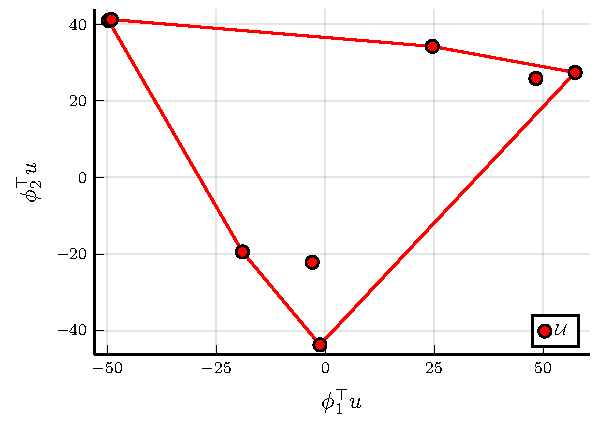
\includegraphics[width=0.45\textwidth]{../notebooks/plots/visual_U.pdf}
    % 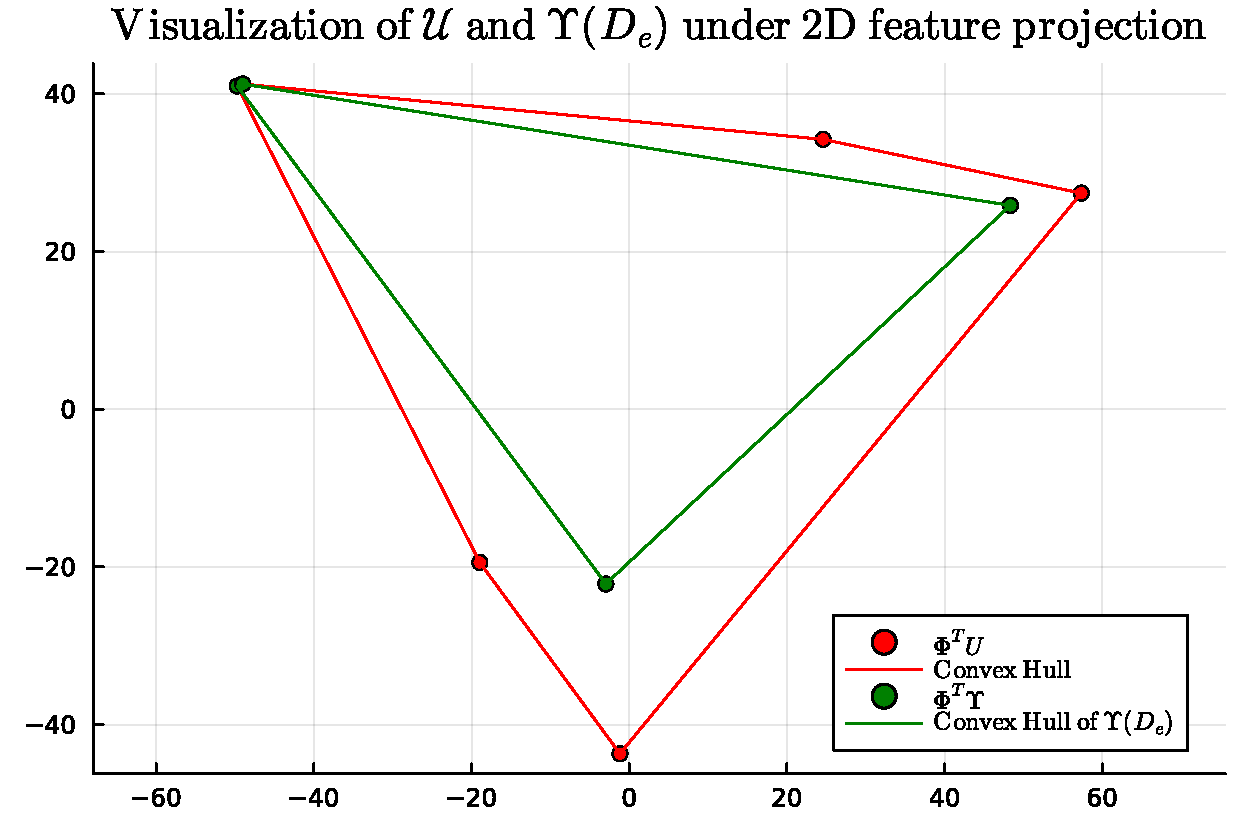
\includegraphics[width=0.35\textwidth]{../notebooks/plots/visual_U_and_Upsilon.pdf}
    % \hspace{0.1\textwidth}
    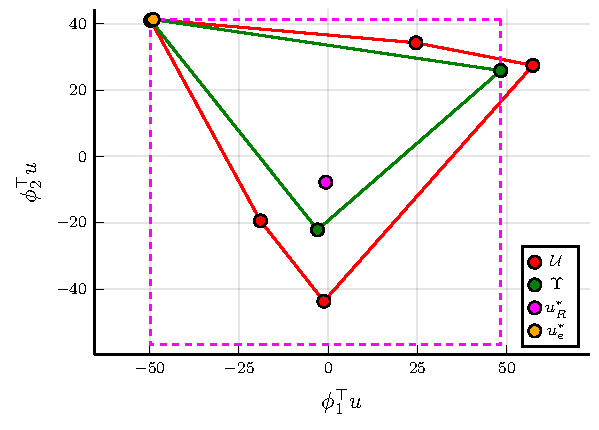
\includegraphics[width=0.45\textwidth]{../notebooks/plots/visual_solve_cheb.pdf}
    %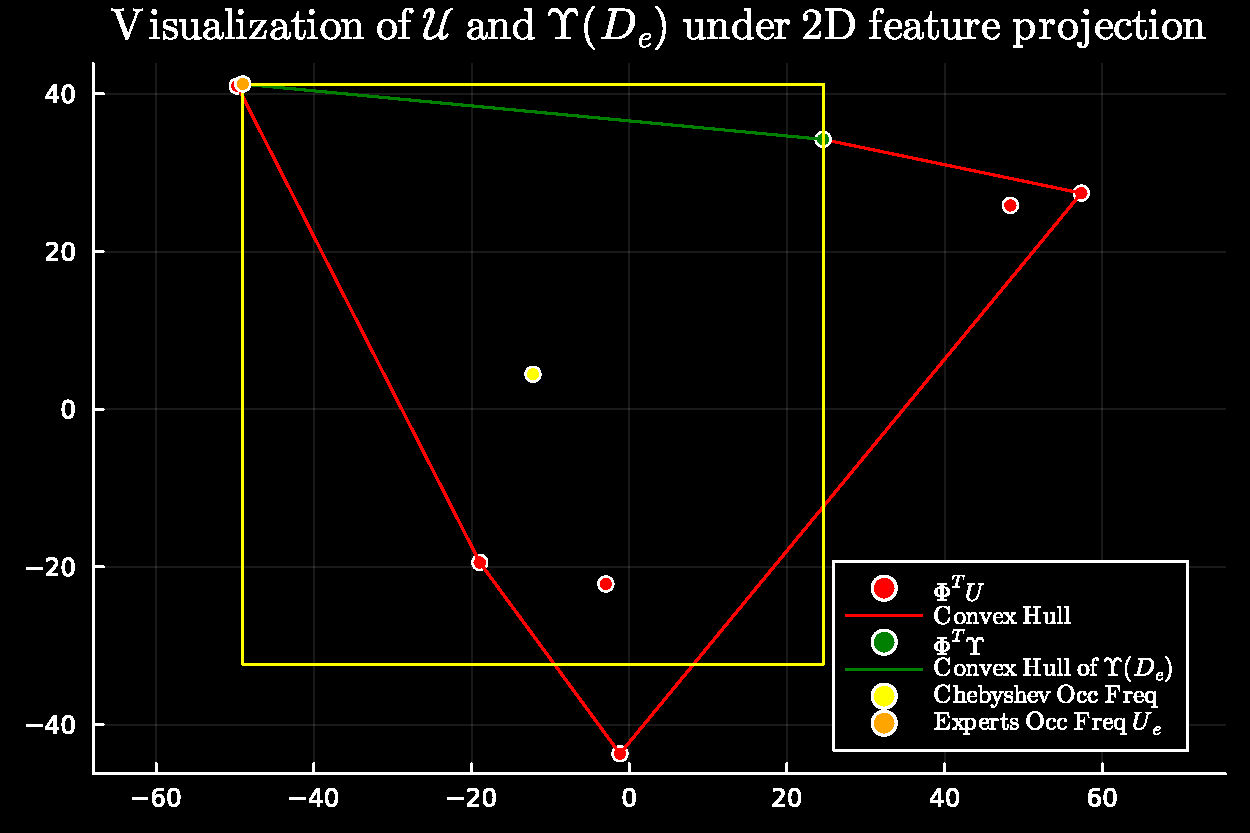
\includegraphics[width=0.35\textwidth]{../notebooks/plots/visual_solve_cheb_outside_upsilon.pdf}
    \caption{Depiction of ROIL solution as a Chebyshev center of the set $\Upsilon$. The dashed line shows the minimum circumscribed $L_{\infty}$ ball.}
    \label{fig:visual_representation_of_ROIL}
\end{figure}

Using the connection with the Chebyshev center problem, \cref{fig:visual_representation_of_ROIL} visualizes ROIL. Consider a small MDP problem with let $\Phi \in \Real^{n \times k}$ with two features $k = 2$. The red polygon represents the set $\Phi\tr \mathcal{U}$ with the points representing extreme points that correspond to deterministic policies. The green polygon represents the set $\Upsilon$ of policies that are consistent with the expert's demonstrations with the points representing extreme points. Note that the extreme points of $\Phi\tr \Upsilon$ are also deterministic policies in $\mathcal{U}$ but do not constitute extreme points of $\Phi\tr \mathcal{U}$.

The relationship to the Chebyshev center problem also offers additional computational insights regarding the choice of $\mathcal{W}$. It is known that popular choices of the distance metric $\| \cdot  \|_{\star}$ in computing the Chebyshev center of a polyhedron are NP-hard. One notable exception is when the distance metric $\| \cdot \|_{\star}$ corresponds to the $L_{\infty}$ norm. Since $L_1$ is the dual norm to the $L_{\infty}$ norm, the choice of $L_1$ in the definition of $\mathcal{W}$ is crucial to obtaining a tractable optimization problem~\cite{Wu2013, Eldar2008}. 


% optimization problem. In the convex optimization literature,
% ~\eqref{eq:robust_IRL_formulation_L1} is a problem of finding the largest minimum
% distance between the edges of polytopes $\mathcal{U}$ and $\Upsilon$. Also known as the Chebyshev center of $\Upsilon$ with respect to $\mathcal{U}$.
% This problem is known to be NP-hard except for certain cases \gersi{citation needed}.

% For those familiar with prior works done by Syed and Schapire~\cite{Syed2008} this is very similar to LPAL and MWAL.
% However, we show that our formulation is more general and can recover the expert exactly in particular cases.


% \begin{equation}
% \label{linProg}
%     \begin{mprog}
%             \minimize{\sigma, \alpha_i, \hat{\alpha}_i \in \Real, \beta_i, \hat{\beta}_i \in \Real^{S}, u \in \Real^{SA}} \sigma
%             \stc -u\tr \Phi_i - \beta_i\tr p_0 \leq \sigma
%             \cs u\tr \Phi_i - \hat{\beta}_i\tr p_0 \leq \sigma
%             \cs \Phi_i + \alpha_i c + A \beta_i \leq 0
%             \cs -\Phi_i + \hat{\alpha}_i c + A \hat{\beta}_i \leq 0
%             \cs i \in 1 \dots k
%             \cs A\tr u = p_0
%             \cs u \geq 0
%     \end{mprog}
% \end{equation}

\section{Theoretical Analysis}
\label{sec:theoretical-analysis}
% \mm{Things to show:
% 	\begin{enumerate}
% 		\item When each state is present in the dataset, then we can compute a policy that has zero worst-case regret
% 		\item What if there is one state that we have not seen, can we bound the regret then?
% 	\end{enumerate}
%  }

In this section, we turn to a theoretical analysis of ROIL. We study the theoretical guarantees of the quality of the solutions computed by ROIL. In particular, we show that, unlike other popular IRL algorithms, ROIL guarantees to recover the expert's policy when demonstrations for all states are available. We also discuss the limitations that arise from the assumption inherent in ROIL formulations and give an approximation error bound in terms of the approximation error bounds.

First, we show that LPAL and GAIL, popular IRL algorithms, suffer from a surprising weakness. The algorithms may not recover the expert's policy even when given demonstrations of deterministic actions for \emph{every} state in a tabular MDP. While it is not a prevalent scenario in practice, it points out that simply adding more demonstrations is insufficient for these methods. We consider the basic version of LPAL and GAIL, which can be stated for tabular features $\Phi = I$ as the following optimization problems:
\begin{equation} \label{eq:lpal-gail}
  \min_{u\in \mathcal{U}}\, \| u - \hat{u}_{\mathrm{e}} \|_{\infty},
  \qquad
  \text{and}
  \qquad
  \min_{u\in \mathcal{U}} \, D_{\mathrm{JS}}(u, \hat{u}_{\mathrm{e}}) - \lambda H(\pi^{u}).
\end{equation}
Here, the first optimization problem represents LPAL~\cite{Syed2008} and the second optimization represents GAIL~\cite[eq.~(15)]{Ho2016}. The distance metric $D_{\mathrm{JS}}$ represents the Jensen-Shannon entropy, and $\lambda \ge 0$ is a regularization parameter. The LPAL optimization problem in~\eqref{eq:lpal-gail} follows immediately from~\eqref{eq:irl-formulation-u} by optimizing over the set of occupancy frequencies. For the sake of consistency with ROIL, we assume that $\mathcal{W}$ is chosen as in~\eqref{eq:r-defintion}. This is a superficial difference from the original LPAL derivations that assume that feature weights are non-negative: $\mathcal{W} = \left\{ w\in \Real^k_+ \mid \| w\|_1 \le  1  \right\}$.
\begin{proposition}
LPAL and GAIL as defined in~\eqref{eq:lpal-gail} may not recover $\pi_{\mathrm{e}}$ even when the demonstrations cover the entire state space: $ \left\{ s\in \mathcal{S} \; \mid \; \exists\; a\in \mathcal{A}, \; (s,a) \in \mathcal{D} \right\} = \mathcal{S}$. 
\end{proposition}
We show the proposition by constructing the following example. 
\begin{example} \label{exm:fail-all}
Consider an MDP with two states and transition probabilities depicted in \cref{fig:example-fail-one}. Suppose that $\pi_{\mathrm{e}}(s) = a_1$ for each $s\in \mathcal{S}$.  The occupancy frequency for this policy is $u\opt_{\mathrm{e}} = \left[ \frac{\epsilon + \gamma - 1}{\epsilon(1-\gamma)}, 0, \frac{1}{\epsilon}\right]$. Assume that the dataset $\mathcal{D} = ( (s_1, a_1), (s_2, a_1) )$ represents the demonstrations; note that the state distribution needs to respect the state distribution of $u_{\mathrm{e}}$. The estimated occupancy frequency will from this dataset will be $\hat{u}_{\mathrm{e}} = \left[\frac{1}{2(1-\gamma)}, 0, \frac{1}{2(1-\gamma)}\right]$ where the elements correspond to $(s_1, a_1), (s_1, a_2), (s_2,a_1)$. The factor $(1-\gamma)^{-1}$ normalizes the occupancy frequencies. The set of occupancy frequencies in this MDP is
\begin{equation} \label{eq:u-definition-example}
  \mathcal{U} = \left\{ \xi \cdot \left[\frac{\epsilon+\gamma-1}{\epsilon(1-\gamma)}, 0, \frac{1}{\epsilon}\right] + (1-\xi) \cdot \left[0,1-\epsilon,\frac{\gamma}{1-\gamma}+\epsilon\right] \;\mid\; \xi \in [0,1]\right\},
\end{equation}
because the set of occupancy frequencies of randomized policies can be represented as a convex hull of the frequencies of deterministic policies. One can then readily verify that $u_{\mathrm{e}}$ does not minimize either one of the objectives in~\eqref{eq:lpal-gail} when $\lambda = 0$. Specifically, choosing $\xi = 0.5$ in~\eqref{eq:u-definition-example} achieves a smaller objective. \Cref{fig:loss_of_LPAL_GAIL} depicts the objective functions in~\eqref{eq:lpal-gail} as a function on $\xi$ in~\eqref{eq:u-definition-example}.
\end{example}

\begin{figure}
  \centering
\begin{center}
	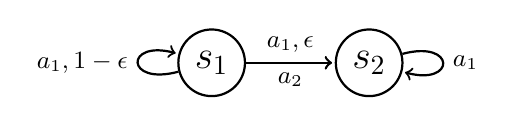
\begin{tikzpicture}[->,shorten >=1pt,auto,node distance=2cm,
			thick,main node/.style={circle,draw,font=\sffamily\Large\bfseries}]

		\node[main node] (1) {$s_1$};
		\node[main node] (2) [right of=1] {$s_2$};

		\path[every node/.style={font=\sffamily\small}]
		(1) edge [loop left] node {$a_1, 1-\epsilon$} (1)
		(1) edge node [below, midway] {$a_2$} (2)
                (1) edge node [above, midway] {$a_1, \epsilon$} (2)
		(2) edge [loop right] node {$a_1$} (2);
	\end{tikzpicture}
\end{center}
  \caption{MDP used in \cref{exm:fail-all}. The edge labels denote the actions and the corresponding transition probabilities (if less than 1).}
  \label{fig:example-fail-one}
\end{figure}


In contrast with LPAL and GAIL, ROIL is guaranteed to recover the expert's policy when provided with demonstrations for all states as the following proposition states.  
\begin{proposition} \label{expert_recovery}
Suppose that $\left\{ s\in \mathcal{S} \; \mid \; \exists\; a\in \mathcal{A}, \; (s,a) \in \mathcal{D} \right\} = \mathcal{S}$. Then $\pi_{\mathrm{e}}$ a minimizer to~\eqref{eq:roil-basic-lp}. Moreover, with the constraint $u\in \Upsilon$ discussed in \cref{sec:incorp-addit-constr}, $u_{\mathrm{e}}$ is also the unique minimizer.
\end{proposition}
\begin{proof}
When $\mathcal{D}$ completely covers the states, $\Pi_{\mathrm{R}}(\mathcal{D}) = \left\{ \pi_{\mathrm{e}} \right\}$ and $\Upsilon = \left\{ u_{\mathrm{e}} \right\}$ by \cref{lemma:occ_freq_matching}. One can readily see that $u_{\mathrm{e}}$ attains $0$ objective in~\eqref{eq:roil-basic-lp}, which is optimal because the regret is lower-bounded by $0$. The uniqueness is immediate because $\Upsilon$ is a singleton.
\end{proof}

\begin{figure}
	\centering
	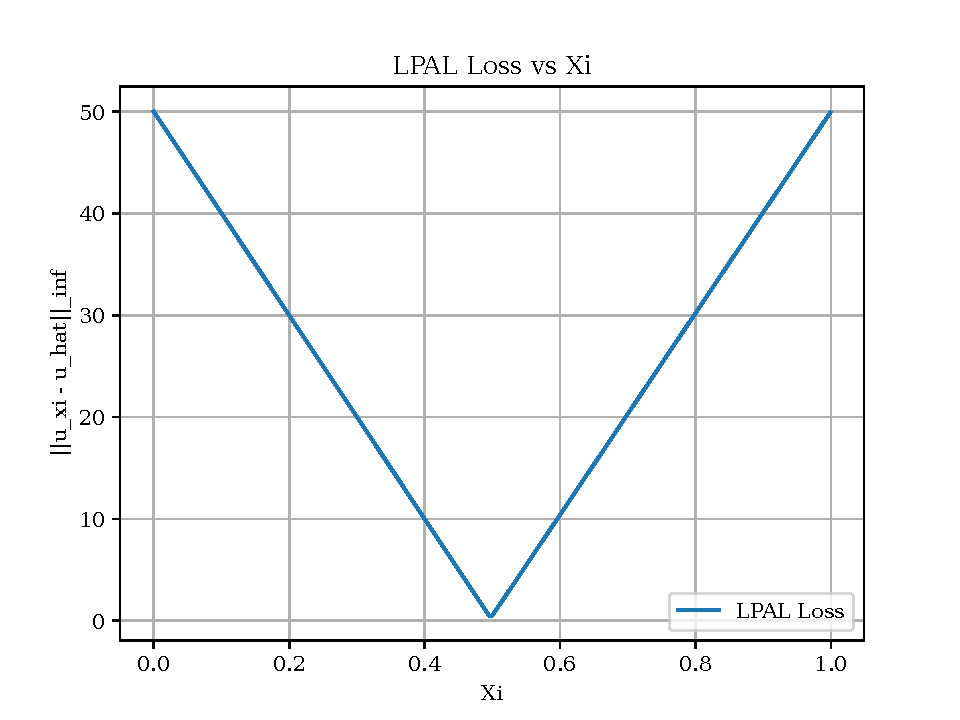
\includegraphics[width=0.45\textwidth]{../src/plots/all_state/lpal_loss.pdf}
	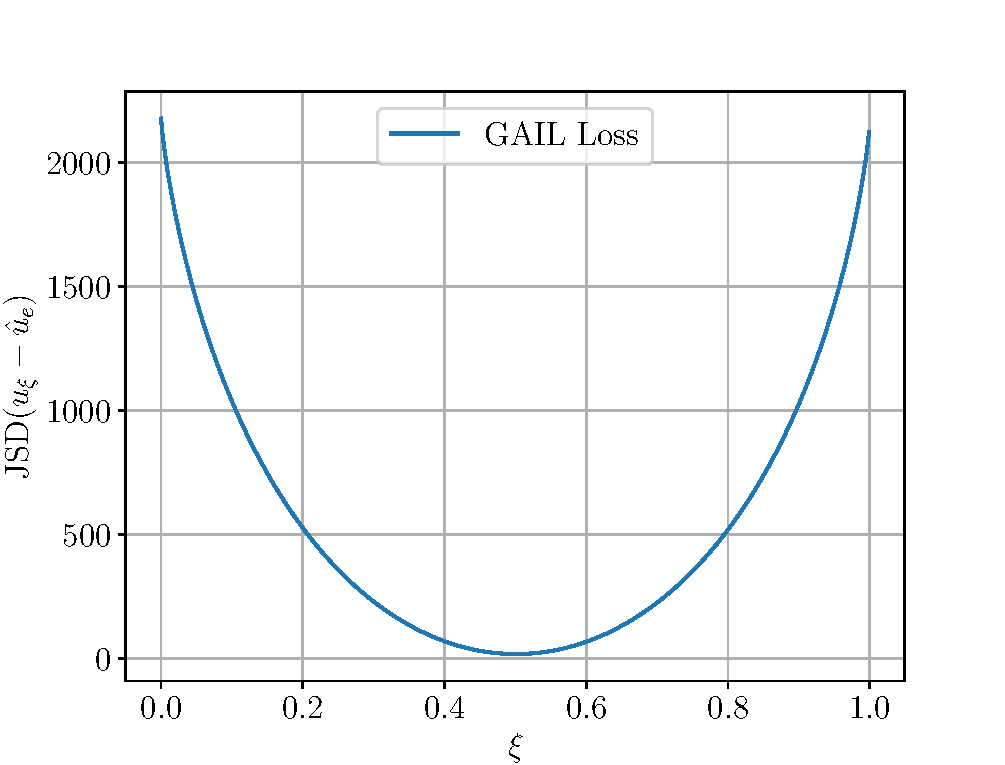
\includegraphics[width=0.45\textwidth]{../src/plots/all_state/gail_loss.pdf}
	\caption{The loss functions of LPAL and GAIL. Here JSD refers to the Jensen-Shannon Divergence which is the loss function minimized by GAIL when the coefficient of the 
 causal entropy term H is zero~\cite{Ho2016}.\mm{this plot needs to use the proper greek letters in the labels.}}
	\label{fig:loss_of_LPAL_GAIL}
\end{figure}

\begin{figure}
  \centering
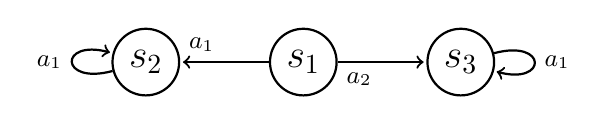
\begin{tikzpicture}[->,shorten >=1pt,auto,node distance=2cm,
            thick,main node/.style={circle,draw,font=\sffamily\Large\bfseries}]

    \node[main node] (1) {$s_1$};
    \node[main node] (2) [left of=1] {$s_2$};
    \node[main node] (3) [right of=1] {$s_3$};

    \path[every node/.style={font=\sffamily\small}]
    (1) edge node [above left] {$a_1$} (2)
    edge node [below left] {$a_2$} (3)
    (2) edge [loop left] node {$a_1$} (2)
    (3) edge [loop right] node {$a_1$} (3);
\end{tikzpicture}
  \caption{An MDP used in \cref{exm:roil-limitations}.}
  \label{fig:roil-fail}
\end{figure}

Recall that ROIL dispenses with the assumption that the states in the demonstrations $\mathcal{D}$ are distributed according to the occupancy frequency. This assumption makes ROIL appropriate in a broader range of off-policy scenarios than competing IRL algorithms. However, the following result shows the limitations arising from ignoring the state distribution assumption in $\mathcal{D}$. The following example demonstrates that even when all but one state is covered by $\mathcal{D}$, ROIL cannot give any guarantees on the regret of the computed policy. 

\begin{example} \label{exm:roil-limitations}
Consider the deterministic MDP depicted in \cref{fig:roil-fail} where $\mathcal{S} = \{s_1, s_2, s_3\}$, $\mathcal{A} = \{a_1, a_2\}$, $p_0 = [1,0,0]$, and $\Phi = r\opt = [0,0,1,1,-1,-1]$. Here, $r\opt$ is the true reward and vectors are ordered as $(s_1,a_1), (s_1, a_2), (s_2,a_1), \dots $. Assume that the expert follows the optimal policy $\pi_{\mathrm{e}}(s) = a_1, \forall s\in \mathcal{S}$ with an occupancy frequency $u_{\mathrm{e}} = [1,0,\nicefrac{\gamma}{1-\gamma},0,0,0]$. However, ROIL fails to find this solution even when demonstrations cover all but one state. Consider the dataset $\mathcal{D} = ((s_2, a_1),  \dots, (s_2, a_1))$. The optimal solution to ROIL is $u = [\nicefrac{1}{2},\nicefrac{1}{2},\nicefrac{\gamma}{2(1-\gamma)},0,\nicefrac{\gamma}{2(1-\gamma)},0]$ which is sub-optimal regardless of how well the estimated $\hat{u}_{\mathrm{e}}$ approximated $u_{\mathrm{e}}$. Using the observed data, ROIL has no evidence supporting taking actions $a_1$ or $a_2 $ in the initial state $s_1$.
\end{example} 

\Cref{exm:roil-limitations} exposes a limitation of ROIL but also hints at how to overcome them. Note that occupancy frequency matching methods, like LPAL~\cite{Syed2008}, may do well in \cref{exm:roil-limitations}. This is because LPAL will use the prevalence of the state $s_2$ in $\mathcal{D}$ to deduce that taking action $a_1$ in $s_1$ is preferable to $a_2$ because it leads to a state that is more common in the dataset. We approach this limitation in \cref{sec:incorp-addit-constr}, where we discuss how one can add distributional assumptions to ROIL. The following theorem shows that with this assumption, we can prove similar approximation bounds to LPAL in the following theorem. 

\begin{theorem} \label{roilRegretBound}
Suppose that $u_{\mathrm{r}}\opt$ is an optimal solution to~\eqref{eq:roil-improved-lp} with some $\epsilon>0$ such that $\hat{\Upsilon}_{\epsilon} \neq \emptyset$ and an occupancy frequency estimate $\hat{u}_{\mathrm{e}}$. Then the regret of $\pi_{\mathrm{r}}\opt  = \pi^{u\opt_{\mathrm{r}}}$ is bounded as
\[
\rho(\pi_{\mathrm{e}}, r) - \rho(\pi_{\mathrm{r}}\opt, r)
\;\leq\;
\| \Phi\tr (\hat{u}_{\mathrm{e}} - u_{\mathrm{e}}) \|_\infty + \eps,
\qquad \forall r\in \mathcal{R}.
\]
Moreover, one can choose $\epsilon$ such that $ \epsilon = \| \Phi\tr (\hat{u}_{\mathrm{e}} - u_{\mathrm{e}}) \|_\infty$.
\end{theorem}
\begin{proof}
The result follows immediately by Holder's inequality, the construction of $\mathcal{W}$, and the triangle inequality as
\begin{align*}
\rho(\pi_{\mathrm{e}}, r) - \rho(\pi_{\mathrm{r}}\opt, r)
  &\le  \max_{r\in\mathcal{R}} r\tr(u_{\mathrm{e}} - u_{\mathrm{r}}\opt)
    = \| \Phi\tr (u_{\mathrm{e}} - u_{\mathrm{R}}(\eps)) \|_\infty
    \leq \| \Phi\tr (u_{\mathrm{e}} - \hat{u}_{\mathrm{e}} + \hat{u}_{\mathrm{e}} - u_{\mathrm{r}}\opt \|_\infty \\
&\leq \| \Phi\tr (u_{\mathrm{e}}-\hat{u}_{\mathrm{e}}) \|_\infty + \| \Phi\tr (\hat{u}_{\mathrm{e}} - u_{\mathrm{R}}\opt) \|_\infty \leq  \| \Phi\tr (u_{\mathrm{e}}-\hat{u}_{\mathrm{e}}) \|_\infty + \eps.
\end{align*}
The last inequality follows from the fact that the $\pi_{\mathrm{r}}\opt  \in \Upsilon$.
\end{proof}

\Cref{roilRegretBound} practically shows that when $\| \Phi\tr (\hat{u}_{\mathrm{e}} - u_{\mathrm{e}}) \|_\infty $ is small, then ROIL with the extensions is guaranteed to find a policy that has a small regret to the expert's policy. We also note that \cref{roilRegretBound} essentially matches the error bounds derived for LPAL~\cite{Syed2008}.


\section{Experimental Results}
\label{sec:experimental-results}


In this section, we study ROIL's behavior numerically on common benchmark problems. We study its performance in on-policy (states distributed according to the policy) and off-policy (states distributed arbitrarily) and compare it with closely related IRL algorithms.

\begin{figure}
	\centering
	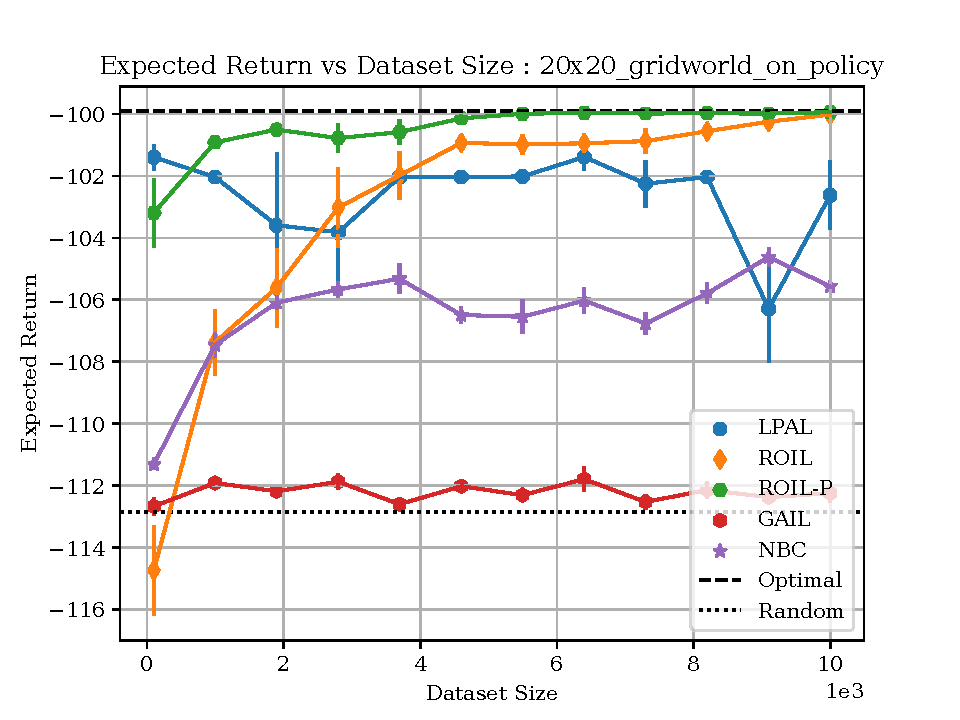
\includegraphics[width=0.45\textwidth]{../src/plots/returns/20x20_gridworld_on_policy_returns.pdf}
	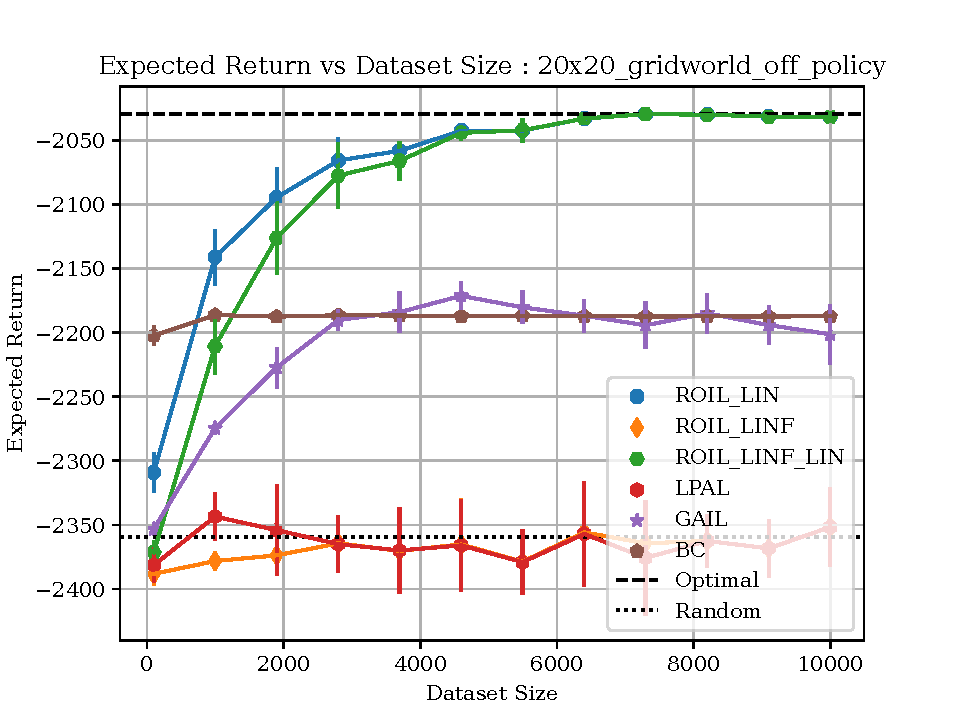
\includegraphics[width=0.45\textwidth]{../src/plots/returns/20x20_gridworld_off_policy_returns.pdf}
	\caption{On and off policy performance of IRL methods on the driving simulator grid world.}
	\label{fig:driving}
\end{figure}

The first domain we use is an instance of the standard grid world problem in which each square is designated a color that represents the feature that is active for the state. The reward is some linear combination of the features for each state. That is, the matrix $\Phi$ represents the state colors and  $r\opt  = \Phi\tr w$ for some $w \in \mathcal{W}$. The features for each action in the state are identical. The agent has a choice of up, down, left, and right as their actions with small noise that takes it to a different neighboring state. The rewards in this domain are generated randomly for each run by sampling $w$ uniformly from $\mathcal{W}$. The expert policy is computed and chosen as the optimal policy for the true (unknown) reward.

The second domain we use is a driving simulator where the agent begins in the bottom row and can go straight up, up and to the left, or up and to the right. At the first row, the actor loops back to the bottom row to simulate a continuous environment. Similarly to the grid world, the driving simulator has some small noise in the transitions. The driving simulator has some motorists on the road, which the actor must avoid, and the left-most and right-most columns are designated as ``guardrails'' where the actor receives negative rewards. The reward in the domain is fixed, and the expert acts optimally for the reward. 

To generate on-policy data, we use the standard protocol in which expert demonstrations are trajectories of a policy. To generate off-policy data, we simulate an expert who aims to give uniform coverage of the states. That is, the expert follows a uniform behavior policy  $\pi_b(s,a) = \nicefrac{1}{\lvert \mathcal{A} \rvert}$, which controls the transition dynamics. The uniform policy $\pi_{\mathrm{b}}$ is only used to generate the states in $\mathcal{D}$ and the true expert $\pi_{\mathrm{e}}$ chooses what action to include in the dataset for the current state.

%This off-policy regime makes it difficult to recover the expert for any method that relies solely on $\hat{u_e}$, which is the estimated occupancy frequency given the expert dataset.

We evaluate two versions of ROIL: The basic ROIL makes no assumptions on $\hat{u}_{\mathrm{e}}$ and solves~\eqref{eq:roil-basic-lp}. The extended \mm{ROILe} solves~\eqref{eq:roil-improved-lp} with $\epsilon$ computed as in~\eqref{eq:minimal-epsilon} with \mm{$\eta = 2$}. We compare these algorithms with two IRL algorithms: LPAL and GAIL. For consistency with our results, we do not impose the constraint $w \ge 0$ used in the original LPAL formulation~\cite{Syed2008}. For the GAIL implementation, we use the original formulation with $\lambda = 0$; we did not find that $\lambda$ had a significant effect on our results. We also compare it with Naive Behavioral Cloning~(NBC). NBC follows the expert's policy in states that are visited but takes random action in states that have not been visited. We did not compare them with other behavioral cloning methods because they require different types of features, which makes them difficult to compare fairly with IRL methods. 



\begin{figure}
	\centering
	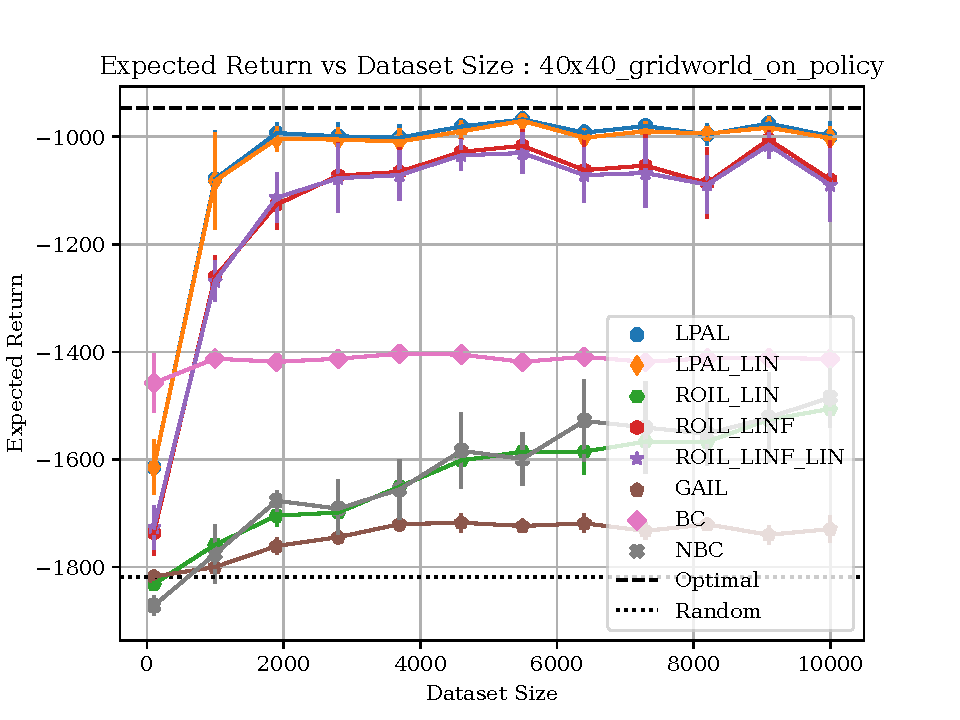
\includegraphics[width=0.45\textwidth]{../src/plots/returns/40x40_gridworld_on_policy_returns.pdf}
	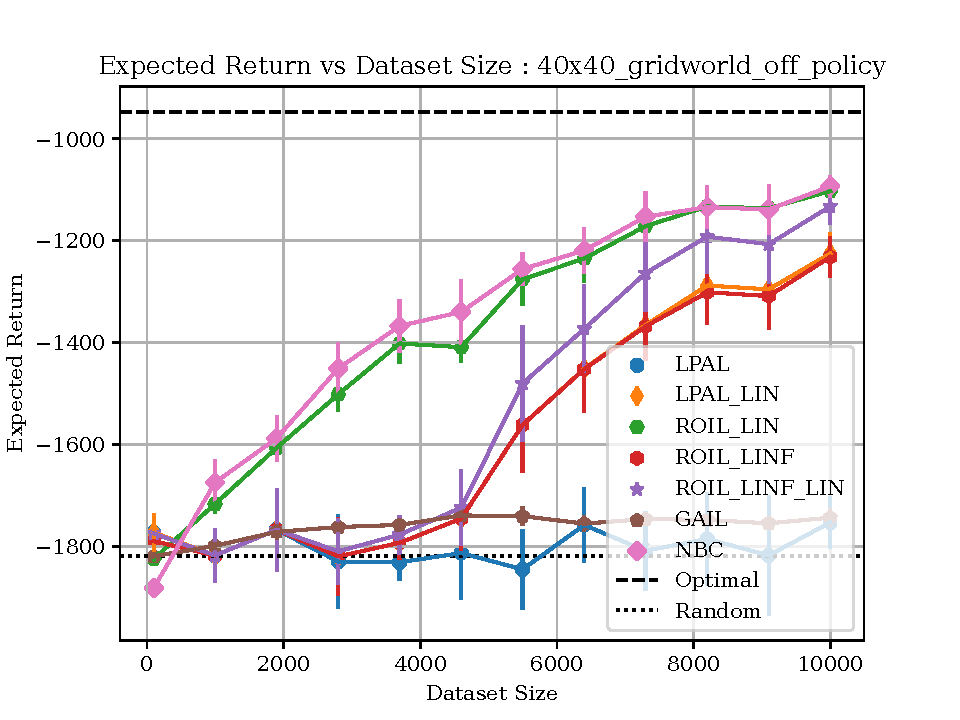
\includegraphics[width=0.45\textwidth]{../src/plots/returns/40x40_gridworld_off_policy_returns.pdf}
	\caption{On and off policy performance of IRL methods on 40x40 grid world}
	\label{fig:grid-40}
\end{figure}


\Cref{fig:driving,fig:grid-40} show the performance of the methods as a function of the number of samples in the demonstrations. The samples are constructed from trajectories sampled from the domain. Each data point is computed as an average of \mm{10} runs of the method. The code used to generate these results is included in the appendix. We do not provide timing data because most of the algorithms are implemented in Python, and the main focus of our methods is on setting where sample complexity and not computation time are the limiting factors. 


The results are not surprising. We see that IRL methods perform very well on policy. This is unsurprising because they match the occupancy frequency, and its estimate improves with increasing samples. However, in the off-policy regime, these methods fail to work well because the estimate $\hat{u}_{\mathrm{e}}$ does not necessarily improve with increasing numbers of samples. ROIL, on the other hand, works well in both settings. We see that ROILe can adaptively choose the error $\epsilon$ that helps it perform well in both on-policy and off-policy settings. 

\section{Conclusion}

We presented a new algorithm for IRL that can handle expert demonstrations gathered for off-policy (or offline) state distributions. This is an important topic that has not received sufficient attention in prior work. We proposed ROIL, a principled and flexible framework for this problem. ROIL minimizes the regret concerning the expert's policy and makes minimal assumptions about the data and the expert. However, the framework can be easily extended to a setting in which one makes more assumptions about the expert and the demonstrations generated. 

There are many avenues for future work. It is important to study whether there are possible refinements of ROIL along the lines described in \cref{sec:incorp-addit-constr} that would significantly impact its performance. We also studied ROIL in a simple tabular setting. Future work needs to study the best ways to generalize these ideas to large problems with continuous states and actions and non-linear function approximators. 




%\bibliographystyle{plain}
\bibliography{irl.bib}

\clearpage
\appendix
\section{Proofs} % of \cref{sec:basic-formulation}}

\begin{lemma}\label{prop:convexity_of_Upsilon}
The set $\Upsilon$ is non-empty, convex, compact, and polyhedral.
\end{lemma}
\begin{proof}
The set is non-empty because $u_{\mathrm{e}} \in \Upsilon$. It is convex and polyhedral from its construction and is compact because it is bounded ($1\tr u \le  \nicefrac{1}{1-\gamma}$) and closed.  
% Since $\mathcal{U}$ is the set of feasible solutions to the dual LP formulation~\cite[Eq.~(6.9.2)]{Puterman1994} it is well known to be polyhedral and convex. To show that the set $\mathcal{U}$ is compact, we need to show that it is bounded. This is true since, $u \in \mathcal{U}$ satisfies $u \ge 0$ by construction, and it is easy to verify that $1\tr u = \frac{1}{1-\gamma}$. Then, the set $\Upsilon$ is an intersection of half-spaces with $\mathcal{U}$ a closed convex set. Any union of closed half-spaces is convex and closed~\cite[eq.~(2.2.1)]{boyd_convex_optimization}.
\end{proof}

\lemmaOccupancyExistance*
\begin{proof}
To show this result, we use the policy to occupancy frequency correspondence~\cite{Puterman1994}. We prove the two implications individually.

Case 1: Prove $u \in \Upsilon   \quad \Rightarrow \quad  \exists
        \pi \in \Pi(\mathcal{D}), \, u = u^{\pi}$,

Given $u \in \Upsilon$, we have that $u^{\pi_{u}} = u$ since $u\in \Upsilon \subseteq \mathcal{U}$ and $p_0 > 0$. Because $u \ge 0$, $u(s,a) = 0$ if $\pi_{\mathrm{e}}(s) \neq 1$ for each $s\in \mathcal{S}$. Moreover, $u(s,a) > 0$ for each $\pi_{\mathrm{e}}(s) = a$ because $\sum_{a\in \mathcal{A}} u(s,a) > 0, \forall s\in \mathcal{S}$ from $p_0 > 0$. Therefore $\pi^u(s,a) = 1 \Leftrightarrow \pi_{\mathrm{r}}(s) = a$ and $u = u^{\pi_{u}}$ and $\pi^u\in \Pi_{\mathrm{R}}(\mathcal{D})$.

Case 2: Prove $\pi \in \Pi_{\mathrm{R}}(\mathcal{D}) \quad \Rightarrow \quad  u_{\pi} \in
        \Upsilon $

        This follows because
\[
 c\tr u^{\pi} = \sum_{s\in \mathcal{S}} \sum_{a\in \mathcal{A}} c(s,a) u(s,a) = 0, 
\]
since $c(s,a) > 0 \Rightarrow \pi(s,a) = 0 \Rightarrow u(s,a) = 0$.
% Given that $\pi \in \Pi_{\mathrm{R}}(\mathcal{D})$, $\pi(a|s) = 1$ for all $(s,a) \in \mathcal{D}$. Therefore, for observed states $s$, $u(s,a) = 0$ for all $a \not= \pi_{\mathrm{e}}(s)$
% since $u(s,a) = \pi(a|s)\sum_{a'}{u_{\pi}(s,a')}$. Then we see that indeed for the $c$ as defined in case 1, $u\tr c = 0$.
\end{proof}

% \roilLp*
% \begin{proof}
%   The result follows from the discussion in \cref{sec:basic-formulation} and by the epigraph formulation of~\eqref{eq:extreme-points-reformulated}.
    % Recall the definition of $\Phi \in \Real^{SA \times K}$ given some arbitrary ordering on $(s,a)$ pairs.
    % \begin{center}
    
    % 	\[\*\Phi\tr \;=\; \begin{bmatrix}
    % 			- & \phi_1\tr & - \\
    % 			- & \phi_2\tr & - \\
    % 			- & \vdots    & - \\
    % 			- & \phi_K\tr & -
    % 		\end{bmatrix}\]
    
    % 	Where $\phi_n = [\phi_n(s,a)\;\;\forall s,a \in S \times A]$ represents the n'th feature evaluated on each $(s,a)$ pair.
    % \end{center}
    
    % We apply a technique called Chebyshev Approximation~\cite{boyd_convex_optimization}(6.1) to equation~\eqref{eq:extreme_points_of_the_IRL_Formulation}.
    % This step can also be seen as writing~\eqref{eq:extreme_points_of_the_IRL_Formulation} in epigraph form.
    
    % \begin{equation}
    % 	\begin{mprog}
    % 		\minimize{u \in \mathcal{U}, \sigma \in \Real} \sigma
    % 		\stc \max_{v \in \Upsilon} |(v - u)\tr \Phi_i| \leq \sigma
    % 		\cs i \in 1 \dots k
    % 	\end{mprog}
    % \end{equation}
    
    % After expanding the absolute value is equivalent to.
    
    % \begin{equation}
    % 	\begin{mprog}
    % 		\minimize{u \in \mathcal{U}, \sigma \in \Real} \sigma
    % 		\stc \max_{v \in \Upsilon} (v - u)\tr \Phi_i \leq \sigma
    % 		\cs \max_{v \in \Upsilon} -(v - u)\tr \Phi_i \leq \sigma
    % 		\cs i \in 1 \dots k
    % 	\end{mprog}
    % \end{equation}
    
    % In order to make the above problem more easily solvable, let us take the dual of the first inner maximization problem.
    
    % \begin{equation}
    % 	\begin{mprog}
    % 		\maximize{v \in \Upsilon} (v - u)\tr \Phi_i
    % 		\cs i \in 1\dots k
    % 	\end{mprog}
    % \end{equation}
    
    % Notice in order to get this into an LP form we need to take the convex set $\Upsilon$ and construct a linear constraint which encapsulates what it means for an element $v \in \Real_+^{SA}$ to be in the set $\Upsilon$. Luckily this is easy to do as $\Upsilon$ is defined as a linear constraint on $\mathcal{U}$. For the sake of simplicity suppose that we consider one fixed $\Phi_i$, and omit the optimization over all $i \in 1\dots k$ for the duration
    % of the dual derivation. But do keep in mind, each feature vector gets its own dual variable.
    
    % \begin{equation}
    % 	\label{eq:primal_IRL_problem}
    % 	\begin{mprog}
    % 		\maximize{v \in \Real_+^{SA}} (v - u)\tr \Phi_i
    % 		\stc c\tr v = 0
    % 		\cs \sum_{a \in \mathcal{A}}(I - \gamma P_a\tr)v(\cdot, a) = p_0
    % 	\end{mprog}
    % \end{equation}
    
    % \begin{equation}
    % 	L(v, \alpha, \beta) = (v - u)\tr \Phi_i + \alpha c\tr v
    % 	+ \beta\tr (\sum_{a \in \mathcal{A}}(I - \gamma P_a\tr)v(\cdot, a) - p_0)
    % \end{equation}
    
    % Writing the summation as a matrix-vector multiplication we have.
    
    % \[\*A \;=\; \begin{bmatrix}
    % 		- & (I - \gamma P_1) & - \\
    % 		- & (I - \gamma P_2) & - \\
    % 		- & \vdots           & - \\
    % 		- & (I - \gamma P_a) & - \\
    % 	\end{bmatrix}\;\in\; \Real^{SA\times S}\]
    
    % \begin{equation}
    % 	\label{eq:rewrite_U_constraint}
    % 	L(v, \alpha, \beta) = (v - u)\tr \Phi_i + \alpha c\tr v
    % 	+ \beta\tr (A\tr v - p_0)
    % \end{equation}
    
    % Notice that we assume that the vector $v \in \Real^{SA}$ iterates over states first before iterating over actions.
    
    % \begin{equation}
    % 	g(\alpha, \beta) = \sup_{v\geq 0} L(v, \alpha, \beta)
    % \end{equation}
    
    % \begin{equation}
    % 	g(\alpha, \beta) = -u\tr \Phi_i - \beta\tr p_0 + \sup_{v\geq 0} (v\tr \Phi_i + \alpha c\tr v + \beta\tr A\tr v)
    % \end{equation}
    
    % \begin{equation}
    % 	g(\alpha, \beta) = -u\tr \Phi_i - \beta\tr p_0 + \sup_{v \geq 0} (\Phi_i\tr + \alpha c\tr + \beta\tr A\tr)v
    % \end{equation}
    
    % Notice that the quantity in the parentheses is linear in $v$, and linear functions are
    % bounded above if and only if their coefficient is 0.
    % Therefore, $g(\alpha, \beta) = \infty$ except for when $\Phi_i + \alpha c + A\beta \leq 0$ in which case
    % $g(\alpha, \beta) = -u\tr \Phi_i - \beta\tr p_0$.
    
    % Now we are ready to define the dual of~\eqref{eq:primal_IRL_problem}.
    % Given that $g(\alpha, \beta)$ is an upper bound on the optimal value of~\eqref{eq:primal_IRL_problem} for feasible $v$, we wish to minimize it.
    
    % \begin{equation}
    % 	\begin{mprog}
    % 		\minimize{\alpha \in \Real, \beta \in \Real^{S}} -u\tr \Phi_i - \beta\tr p_0
    % 		\stc \Phi_i + \alpha c + A\beta \leq 0
    % 	\end{mprog}
    % \end{equation}
    
    % Recall the formulation of the Chebyshev Center.
    % \begin{equation}
    % 	\begin{mprog}
    % 		\minimize{u \in \mathcal{U}, \sigma \in \Real} \sigma
    % 		\stc \max_{v \in \Upsilon} (v - u)\tr \Phi_i \leq \sigma
    % 		\cs \max_{v \in \Upsilon} -(v - u)\tr \Phi_i \leq \sigma
    % 		\cs i \in 1 \dots k
    % 	\end{mprog}
    % \end{equation}
    
    % Now derive a similar result for the second maximization using the same method as above and substitute.
    % Recall that each feature-vector has its own unique dual variables.
    
    % \begin{equation}
    % 	\begin{mprog}
    % 		\minimize{u\in\mathcal{U}, \sigma\in\Real} \sigma
    % 		\stc \min_{\alpha_i \in \Real, \beta_i \in \Real^{S}} -u\tr \Phi_i - \beta_i\tr p_0 \leq \sigma
    % 		\cs \Phi_i + \alpha_i c + A \beta_i \leq 0
    % 		\cs \min_{\hat{\alpha}_i \in \Real, \hat{\beta}_i \in \Real^{S}} u\tr \Phi_i - \hat{\beta}_i\tr p_0 \leq \sigma
    % 		\cs -\Phi_i + \hat{\alpha}_i c + A \hat{\beta}_i \leq 0
    % 		\cs i \in 1 \dots k
    % 	\end{mprog}
    % \end{equation}
    
    % \begin{equation}
    % 	\begin{mprog}
    % 		\label{eq:semi_fininished_LP}
    % 		\minimize{u\in\mathcal{U}, \sigma, \alpha_i, \hat{\alpha}_i \in \Real, \beta_i, \hat{\beta}_i \in \Real^{S}} \sigma
    % 		\stc -u\tr \Phi_i - \beta_i\tr p_0 \leq \sigma
    % 		\cs u\tr \Phi_i - \hat{\beta}_i\tr p_0 \leq \sigma
    % 		\cs \Phi_i + \alpha_i c + A \beta_i \leq 0
    % 		\cs -\Phi_i + \hat{\alpha}_i c + A \hat{\beta}_i \leq 0
    % 		\cs i \in 1 \dots k
    % 	\end{mprog}
    % \end{equation}
    
    % And now for the final push, notice that~\eqref{eq:semi_fininished_LP} is not an LP,
    % because of the nonlinear (yet convex) minimization over $u\in\mathcal{U}$. To remedy this notice
    % how we re-wrote the definition of $\mathcal{U}$ in~\eqref{eq:rewrite_U_constraint}. This leads us to the
    % LP formulation of the Chebyshev Center.
    % \gersi{TODO go back and explain why the $A^{T}v$ constraint makes sense}
    
    % \begin{equation}
    % 	\begin{mprog}
    % 		\minimize{\sigma, \alpha_i, \hat{\alpha}_i \in \Real, \beta_i, \hat{\beta}_i \in \Real^{S}, u \in \Real^{SA}} \sigma
    % 		\stc -u\tr \Phi_i - \beta_i\tr p_0 \leq \sigma
    % 		\cs u\tr \Phi_i - \hat{\beta}_i\tr p_0 \leq \sigma
    % 		\cs \Phi_i + \alpha_i c + A \beta_i \leq 0
    % 		\cs -\Phi_i + \hat{\alpha}_i c + A \hat{\beta}_i \leq 0
    % 		\cs i \in 1 \dots k
    % 		\cs A\tr u = p_0
    % 		\cs u \geq 0
    % 	\end{mprog}
    % \end{equation}
% \end{proof}


% \section{Proofs of \cref{sec:geom-intu-reduct} }

% \chebeyshevRegret*
% \begin{proof}
% 	For the sake of contradiction,
% 	assume there exists some $\pi' \in \Pi$ such that
% 	\[
% 		\max_{r\in \mathcal{R}} \max_{\pi \in \Pi_{R}(\mathcal{D})}
% 		\left(\rho(\pi,r) - \rho(\pi', r)\right) < \max_{r\in \mathcal{R}}
% 		\max_{\pi \in \Pi_{R}(\mathcal{D})}
% 		\left(\rho(\pi, r) - \rho(\hat{\pi}, r)\right)
% 	\]
% 	After algebraic manipulation, we have
% 	\begin{align*}
% 		\max_{r\in \mathcal{R}} \max_{\pi \in \Pi_{R}
% 			(\mathcal{D})} u_{\pi}\tr r - u_{\pi'}\tr r
% 		 & < \max_{r\in \mathcal{R}}
% 		\max_{\pi \in \Pi_{R}
% 			(\mathcal{D})} u_{\pi}\tr r - u_{\hat{\pi}}
% 		\tr r                                              \\
% 		\max_{r\in \mathcal{R}} \max_{\pi \in \Pi_{R}(\mathcal{D})}
% 		(u_{\pi} - u_{\pi'})\tr r
% 		 & < \max_{r\in \mathcal{R}}
% 		\max_{\pi \in \Pi_{R}(\mathcal{D})}
% 		(u_{\pi} - u_{\hat{\pi}})\tr r
% 		\\
% 		\max_{w\in \mathcal{W}} \max_{v \in \Upsilon} (v - u_{\pi'})\tr \Phi w
% 		 & < \max_{w\in \mathcal{W}} \max_{v \in \Upsilon}
% 		(v - u_{\hat{\pi}})\tr \Phi w
% 	\end{align*}
% 	Here, $u_{\pi}$, $u_{\pi'}$, and $u_{\hat{\pi}}$
% 	are the occupancy frequencies of their respective policies.

% 	Notice the change in the maximization objectives.
% 	We assume that $r = \Phi\tr w$ for some $w \in \mathcal{W}$,
% 	thus the maximization over $\mathcal{R}$ is equivalent to the maximization
% 	over $\mathcal{W}$ of $\Phi\tr w$.
% 	Secondly, by the occupancy frequency correspondence~\cite{Puterman1994}, the
% 	maximization over $\Pi_{\mathrm{R}}(\mathcal{D})$ is equivalent to the maximization over
% 	$\Upsilon$.
% 	Since $u_{\hat{\pi}} \in \arg\min_{u \in \mathcal{U}} \max_{w \in \mathcal{W}} \max_{v \in \Upsilon} {(v - u)}^T \Phi w$,
% 	this is a contradiction with the optimality of $\hat{\pi}$,
% 	therefore $\pi'$ cannot achieve less regret than $\hat{\pi}$.
% \end{proof}

% \paragraph{Relationship With LPAL, Syed and Schapire~\cite{Syed2008}}

% Theorem 5 of the LPAL paper~\cite{Syed2008} provides a bound on the performance of the policy returned by LPAL.
% In this section, we would like to provide insight into this bound using the notation of this paper.

% \begin{restatable}[LPAL bound]{theorem}{LPAL}
% \label{thm:LPAL}
% 	Let $\pi_{lp}$ be the policy returned by LPAL then
% 	\[V(\pi_{lp}) \geq V(\pi_{\mathrm{e}}) + v^* - 2\eps\]
% 	or equivalently expressed using occupancy frequencies
% 	\[u_{lp}\tr r \geq u_{\mathrm{e}}\tr r + v^* - 2\eps\]

% 	Where $\eps = \lvert\lvert \hat{u}_{\mathrm{e}}\tr \Phi - u_e\tr \Phi\rvert\rvert_*$
% \end{restatable}
% \begin{proof}
% 	Begin with the definitions
% 	\[
% 		u^* = \arg\min_{u \in \mathcal{U}} \lvert\lvert u\tr \Phi - \hat{u_{\mathrm{e}}}\tr \Phi \rvert\rvert_*
% 	\]
% 	\[
% 		v^* = - \lvert\lvert \Phi\tr u^* - \Phi\tr \hat{u_{\mathrm{e}}} \rvert\rvert_*
% 	\]
% 	Given that we wish to bound $V(\pi_{lp}) - V(\pi_{\mathrm{e}})$ lets begin with the definition of $V(\cdot)$.
% 	\[V(\pi_{lp}) - V(\pi_{\mathrm{e}}) = u_{lp}\tr r - u_e\tr r\]
% 	Both LPAL and our paper assumes that $r = \Phi\tr w$ for some $w \in \mathcal{W} = \Real_{1}$ LPAL calls the columns of $\Phi$ basis
% 	reward vectors, while we call them features but they are the same, save for notation.
% 	\[\geq \min_{w \in \mathcal{W}}(u_{lp}\tr \Phi w - u_{\mathrm{e}}\tr \Phi w) =- \max_{w \in \mathcal{W}}(u_e\tr \Phi - u_{lp}\tr \Phi)w \]
% 	Applying the definition of the dual norm with respect to $\mathcal{W}$
% 	\[= -\lvert\lvert u_{\mathrm{e}}\tr \Phi - u_{lp}\tr \Phi \rvert\rvert_*\]
% 	Now we apply the triangle inequality by adding 0
% 	\[= -\lvert\lvert u_{\mathrm{e}}\tr \Phi - \hat{u}_e + \hat{u}_e - u_{lp}\tr \Phi \rvert\rvert_*\]
% 	\[\geq -\lvert\lvert u_{\mathrm{e}}\tr \Phi - \hat{u}_e\rvert\rvert_* - \lvert\lvert \hat{u}_e - u_{lp}\tr \Phi \rvert\rvert_* = -\eps - \lvert\lvert \hat{u}_e - u_{lp}\tr \Phi \rvert\rvert_* \]
% 	\[\geq -\eps - \lvert\lvert \hat{u}_{\mathrm{e}}\tr \Phi - \Phi\tr u^*\rvert\rvert_*\]
% 	\[= -\eps - \lvert\lvert \hat{u}_{\mathrm{e}}\tr \Phi - u_e\tr\Phi + u_e\tr\Phi - \Phi\tr u^*\rvert\rvert_*\]
% 	\[\geq -\eps - \lvert\lvert \hat{u}_{\mathrm{e}}\tr \Phi - u_e\tr\Phi\rvert\rvert_* - \lvert\lvert u_e\tr\Phi - \Phi\tr u^*\rvert\rvert_*\]
% 	\[= -2\eps - \lvert\lvert u_{\mathrm{e}}\tr\Phi - \Phi\tr u^*\rvert\rvert_* = -2\eps + v^*\]
% \end{proof}
\end{document}
%%% Local Variables:
%%% mode: LaTeX
%%% TeX-master: t
%%% End:
